%ARCHITETTURA APP ESTERNA
\subsection{Applicazione esterna alla piattaforma Grafana}
Per poter visualizzare la suddivisione delle componenti dell'applicazione esterna e le dipendenze che sussistono tra loro ad alto livello, viene riportato il diagramma dei Package in allegato nel file \textit{diagramma-package-app.png}.
	\subsubsection{Progettazione architetturale}
	Abbiamo deciso di utilizzare un design pattern architetturale Model-View-ViewModel (MVVM) perché si adatta bene alle tecnologie che vengono utilizzate ovvero React ed Electron. In particolare, come si può vedere dalla figura seguente, la View invia dati a ViewModel che a sua volta fornisce delle risposte che permettono di tenere la vista sempre aggiornata. Questo scambio di dati è asincrono ed è fornito interamente da Electron. Inoltre abbiamo la comunicazione tra ViewModel e Model che avviene con la richiesta di esecuzione delle operazioni da parte del ViewModel e la conseguente risposta da parte del Model. Anche questo scambio di messaggi è asincrono ed è implementato da un meccanismo di callback.
	\mbox{}
	\begin{landscape}
		\begin{figure}
			\begin{figure} [H]
				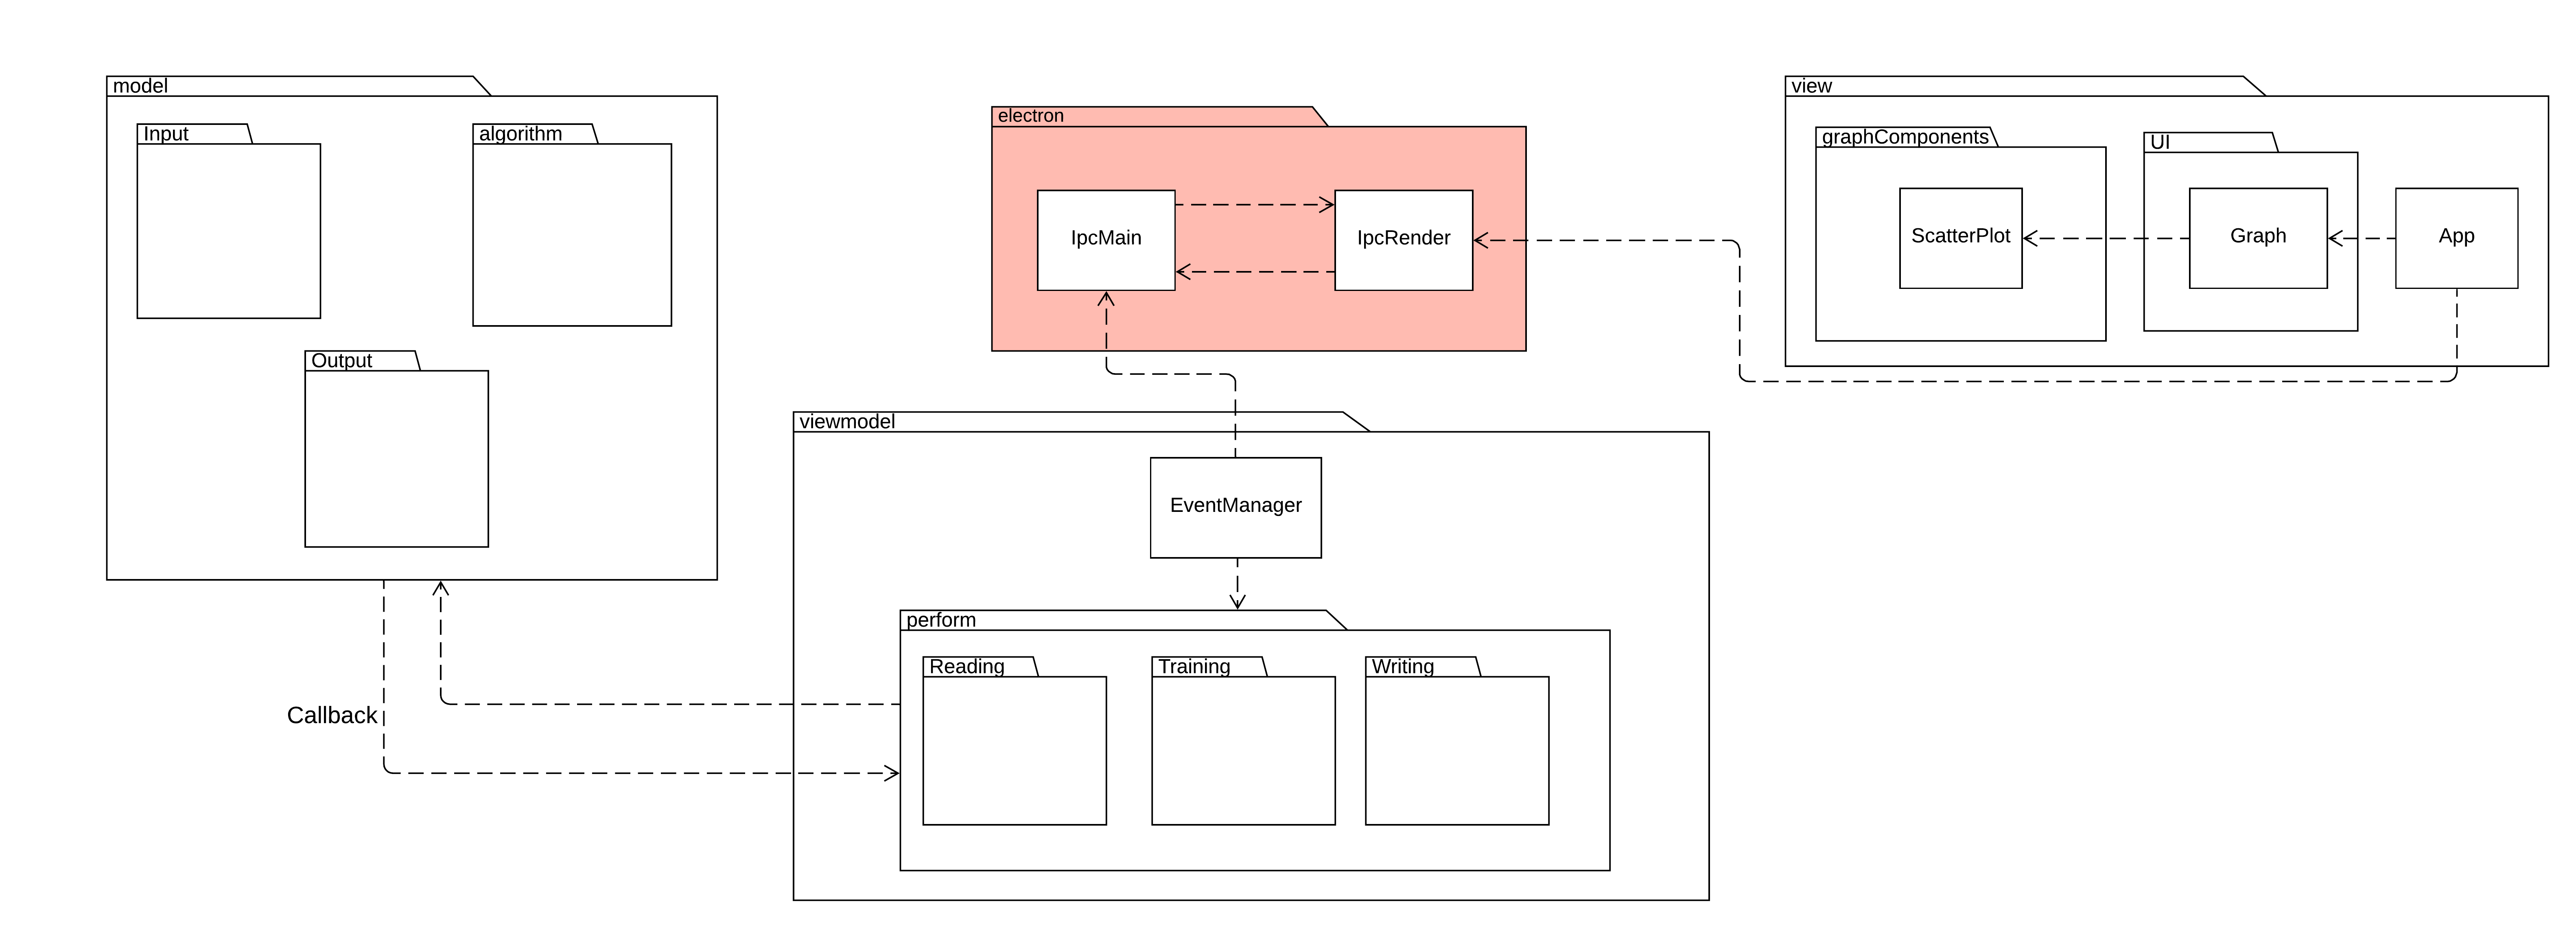
\includegraphics[width=\linewidth]{./img/Diagrammi/architettura-app.png}
				\caption{Diagramma dell'architettura dell'applicazione}
			\end{figure}
		\end{figure}
	\end{landscape}
	Analizzando i componenti, la nostra architettura è così strutturata: 
	\begin{itemize}
		\item \textbf{Model}: modulo che gestisce la business logic. Più in dettaglio esegue l'addestramento dei dati attraverso gli algoritmi di predizione e le operazioni di input/output dei file;
		\item \textbf{View}: modulo che gestisce la presentazione dei dati attraverso React;
		\item \textbf{ViewModel}: modulo che gestisce il binding tra View e Model con un meccanismo detto two-way-data-binding.
	\end{itemize}
	\subsubsection{Progettazione di dettaglio}
		Di seguito viene descritta in dettaglio la progettazione dell'applicazione. In allegato viene fornito il file \textit{diagramma-classi-app.png} contenente l'intero diagramma delle classi.
		\paragraph{Model} \mbox{} 
		\paragraph*{Algorithm} \mbox{} \\[1mm]
		Per la gestione degli algoritmi di addestramento abbiamo scelto di implementare due classi distinte \textit{SvmTrainer} e \textit{RlTrainer} che hanno una dipendenza di tipo composizione dalle rispettive classi delle librerie e del tipo di risultato ottenuto.
		All'interno di ognuna di esse viene fornita la possibilità di addestrare l'algoritmo e di calcolarne gli indici di qualità.
		\mbox{}
		\begin{landscape}
			\begin{figure}
				\begin{figure} [H]
					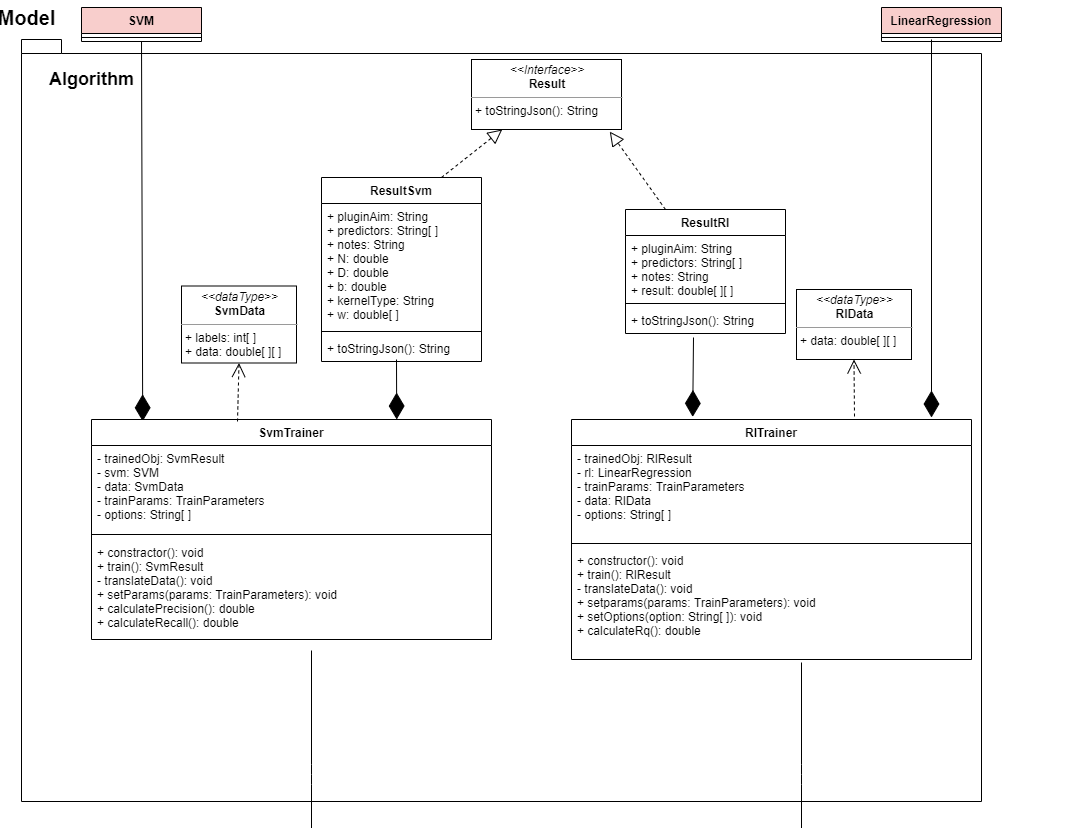
\includegraphics[width=\linewidth]{./img/Diagrammi/algorithm-app.png}
					\caption{Diagramma delle classi per gli algoritmi nel Model}
				\end{figure}
			\end{figure}
		\end{landscape}
		\paragraph*{Read} \mbox{} \\[1mm]
		Abbiamo riscontrato nella gestione dell'input che, indipendentemente dalla tipologia di file ricevuto, l'algoritmo per eseguire la lettura di quest'ultimo ha uno scheletro comune. È stato quindi deciso di implementare il design pattern template method.
		La classe astratta \textit{Read} implementa il metodo \textit{ReadFile(path, callback)} che rappresenta la parte comune dell'algoritmo di lettura da file. Inoltre contiene il metodo astratto \textit{parser(data, callback)} che invece rappresenta la trasformazione del contenuto del file sulla base della sua estensione e perciò viene implementato nelle classi concrete che estendono \textit{Read}. Nel nostro caso esse sono \textit{ReadCsv} e \textit{ReadJson}.
		\mbox{}
		%\begin{landscape}
			%\begin{figure}
				\begin{figure} [H]
					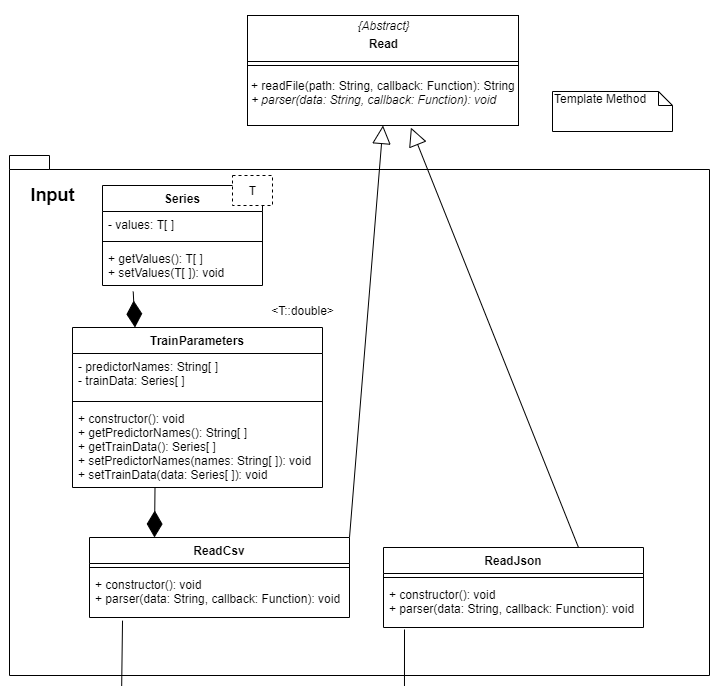
\includegraphics[width=\linewidth]{./img/Diagrammi/read-app.png}
					\caption{Diagramma delle classi per la Read nel Model}
				\end{figure}
			%\end{figure}
		%\end{landscape}
		\paragraph*{Write} \mbox{} \\[1mm]
		Anche nella gestione dell'output abbiamo riscontrato che, indipendentemente dalla tipologia di file su cui scrivere, l'algoritmo per eseguire la scrittura di quest'ultimo ha uno scheletro comune. È stato quindi deciso di implementare il design pattern template method.
		La classe astratta \textit{Write} implementa il metodo \textit{writeToDisk(path, name, data, notes, callback)} che rappresenta la parte comune dell'algortimo di scrittura su file. Inoltre contiene il metodo astratto \textit{parser(data, callback)} che invece rappresenta la trasformazione dell'oggetto che vogliamo scrivere sul file nel formato corretto. Nel nostro caso abbiamo implementato la classe concreta \textit{WriteJson} ma è estendile a tutti i formati di file desiderati estendendo \textit{Write}.
		\mbox{}
		%\begin{landscape}
		%	\begin{figure}
				\begin{figure} [H]
					\begin{center}
						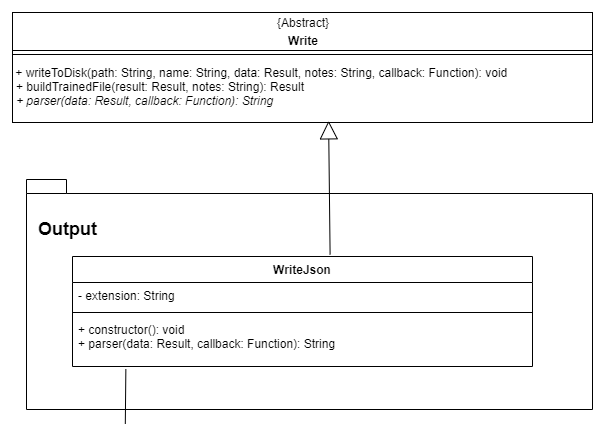
\includegraphics[width=120mm]{./img/Diagrammi/write-app.png}
					\end{center}
					\caption{Diagramma delle classi per la Write nel Model}
				\end{figure}
		%	\end{figure}
		%\end{landscape}

		\paragraph{View} \mbox{} \\[1mm]
		La View è realizzata attraverso dei componenti di React contenuti nella classe principale \textit{App} attraverso una dipendenza di tipo composizione. Grazie all'estensione della classe \textit{Component} di React, otteniamo il metodo \textit{render()} che renderizza i componenti visualizzandoli nell'interfaccia utente.
		Infine per l'implementazione del grafico di addestramento, utilizziamo la libreria D3.
		\mbox{}
		%\begin{landscape}
		%	\begin{figure}
				\begin{figure} [H]
					\begin{center}
						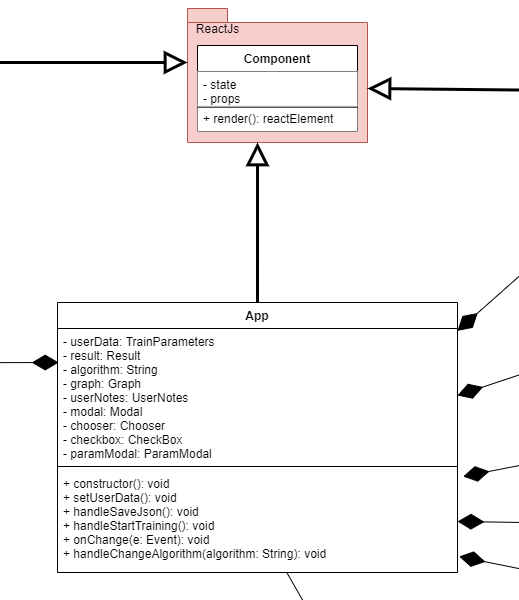
\includegraphics[width=100mm]{./img/Diagrammi/view-app.png}
					\end{center}
					\caption{Diagramma delle classi della View}
				\end{figure}
		%	\end{figure}
		%\end{landscape}
	
		\paragraph{ViewModel} \mbox{} \\[1mm]
		La ViewModel contiene i dati da visualizzare nella vista e le trasformazioni per richiamare le operazioni da eseguire nel modello.
		In particolare è legato alla View tramite Electron che gestisce la loro comunicazione in modo asincrono appoggiandosi al nostro componente \textit{EventManager} e al Model attraverso il meccanismo asincrono di callback.
		Abbiamo riscontrato la necessità di implementare il design pattern strategy in tre casi diversi:
		\paragraph*{Algorithm} \mbox{}
		\begin{itemize}
			\item \textbf{ProcessTraining}: è una classe concreta che rappresenta il context. In essa viene scelto quale algoritmo addestrare sulla base dei dati ricevuti ed ha una dipendenza di tipo aggregazione dall'interfaccia \textit{PerformTraining};
			\item \textbf{PerformTraining}: è un'interfaccia che rappresenta la strategia astratta. Essa definisce il contratto da rispettare per le classi che implementano il process degli algoritmi di addestramento;
			\item \textbf{PerformTrainingSvm}: è una classe concreta che implementa \textit{PerformTraining} e rappresenta il componente che esegue la trasformazione ed il controllo dei dati per richiamare correttamente l'algortimo di addestramento SVM\glosp nel Model.
			\item \textbf{PerformTrainingRl}: è una classe concreta che implementa \textit{PerformTraining} e rappresenta il componente che esegue la trasformazione ed il controllo dei dati per richiamare correttamente l'algortimo di addestramento RL\glosp nel Model.
		\end{itemize}
		\mbox{}
		\begin{landscape}
			\begin{figure}
				\begin{figure} [H]
					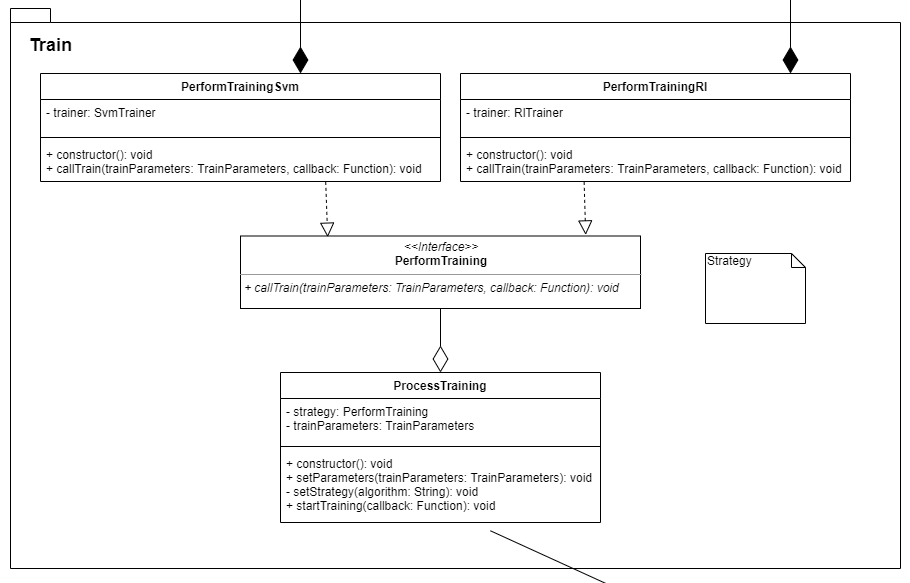
\includegraphics[width=\linewidth]{./img/Diagrammi/ViewModel-train-app.png}
					\caption{Diagramma delle classi per il training nel ViewModel}
				\end{figure}
			\end{figure}
		\end{landscape}
		Per spiegare meglio l'insieme di azioni compiute al fine di processare i dati per eseguire l'addestramento degli algoritmi, illustriamo un diagramma di sequenza che prende in esame SVM\glo. Per gli altri algoritmi il procedimento è simile.
		\mbox{}
		\begin{landscape}
			\begin{figure}
				\begin{figure} [H]
					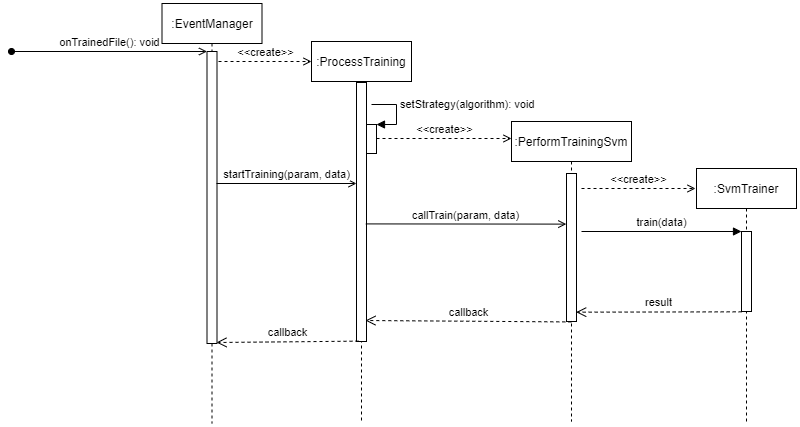
\includegraphics[width=\linewidth]{./img/Diagrammi/ds-app.png}
					\caption{Diagramma di sequenza di processo dei dati per SVM}
				\end{figure}
			\end{figure}
		\end{landscape}
		\paragraph*{Read} \mbox{}
		\begin{itemize}
			\item \textbf{ProcessReading}: è una classe concreta che rappresenta il context. In essa viene scelta la tipologia di file da leggere sulla base dei dati ricevuti ed ha una dipendenza di tipo aggregazione dall'interfaccia \textit{PerformReading};
			\item \textbf{PerformReading}: è un'interfaccia che rappresenta la strategia astratta. Essa definisce il contratto da rispettare per le classi che implementano la lettura da file;
			\item \textbf{PerformReadingCsv}: è una classe concreta che implementa \textit{PerformReading} e rappresenta il componente che esegue le trasformazioni necessarie per richiamare la correttamente l'algoritmo di lettura di un file Csv del Model;
			\item \textbf{PerformReadingJSon}: è una classe concreta che implementa \textit{PerformReading} e rappresenta il componente ch esegue le trasformazioni necessarie per richiamare la correttamente l'algoritmo di lettura di un file Json del Model.
		\end{itemize}
		\mbox{}
		%\begin{landscape}
		%	\begin{figure}
				\begin{figure} [H]
					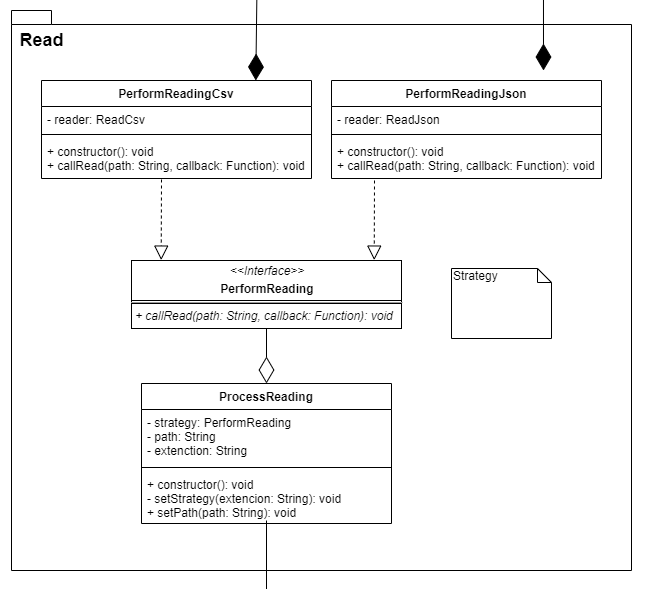
\includegraphics[width=\linewidth]{./img/Diagrammi/ViewModel-read-app.png}
					\caption{Diagramma delle classi per la Read nel ViewModel}
				\end{figure}
		%	\end{figure}
		%\end{landscape}
		\paragraph*{Writing} \mbox{} \\[1mm]
		\begin{itemize}
			\item \textbf{ProcessWriting}: è una classe concreta che rappresenta il context. in essa viene scelta la tipologia di file su cui scrivere in base ai dati ricevuti ed ha una dipendenza di tipo aggregazione dall'interfaccia \textit{PerformWriting};
			\item \textbf{PerformWriting}: è un'interfaccia che rappresenta la strategia astratta. Essa definisce il contratto da rispettare per le classi che implementano la lettura da file;
			\item \textbf{PerformWritingJson}: è una classe concreta che implementa \textit{PerformWriting} e rappresenta il componente che esegue le trasformazioni necessarie per richiamare correttamente l'algoritmo di scrittura di un file Json del Model.
		\end{itemize}
		\mbox{}
		%\begin{landscape}
		%	\begin{figure}
				\begin{figure} [H]
					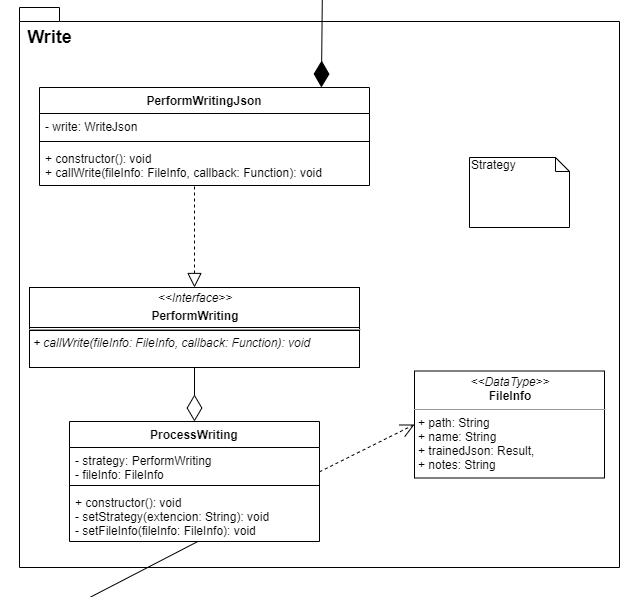
\includegraphics[width=\linewidth]{./img/Diagrammi/ViewModel-write-app.png}
					\caption{Diagramma delle classi per la Write nel ViewModel}
				\end{figure}
		%	\end{figure}
		%\end{landscape}
		
